\documentclass{article}
\usepackage[a4paper, top=2cm, bottom=2cm, left=3.5cm, right=3.5cm]{geometry}
\usepackage{graphicx} % Required for inserting images
\usepackage{algorithm}
\usepackage{algorithmic}
\usepackage{amsmath}

\title{Hybrid Distributed Sort with Bitonic Interchanges}
\author{Georgios Rousomanis \\
Department of Electrical and Computer Engineering \\
Aristotle University of Thessaloniki \\
\texttt{rousoman@ece.auth.gr}}
\date{July 2025}


\begin{document}

\maketitle

\section{Introduction}

Sorting is one of the most fundamental operations in computer science, with broad applications in data 
processing, scientific computing, and distributed systems. As dataset sizes continue to grow, leveraging 
parallel and distributed architectures becomes essential to achieve performance and scalability. 
Bitonic Sort is a well-known comparison-based sorting algorithm that is especially amenable to 
parallelization due to its regular structure and predictable communication pattern.

This project focuses on the implementation and benchmarking of a hybrid distributed sorting algorithm that 
employs Bitonic Sort for inter-process sorting. The dataset to be sorted consists of $N = 2^{p+q}$ integers,
distributed across $2^p$ MPI processes. Each process receives a chunk of $2^q$ elements. The algorithm first 
performs a local sort and then enters a series of bitonic merging phases that involve both local and 
inter-process communication steps.

The goal of this work is to evaluate the performance of the parallel Bitonic Sort implementation under various 
configurations. We study how execution time and communication cost scale with the number of processes, data size, 
and the degree of communication granularity controlled by the parameter $s$, which represents the buffer splitting
depth. Benchmarks are conducted on a high-performance computing cluster, and results are visualized to identify 
performance trends and bottlenecks.

\section{Algorithm Overview}

The implemented algorithm is a hybrid distributed sorting method that combines local sorting with 
parallel Bitonic merging across multiple MPI processes. Each of the $2^p$ MPI processes receives a 
block of $2^q$ integers. The parameter $s$ controls the communication buffer size, dividing each local 
array into $2^{q-s}$ chunks for non-blocking communication during the pairwise exchange phase.

\subsection{Stages of the Algorithm}
The algorithm proceeds in three main stages:
\begin{enumerate}
    \item \textbf{Initial Alternating Sort:}  
    Each process locally sorts its data. Processes with even ranks sort in ascending order, while processes 
    with odd ranks sort in descending order, thus preparing a ``bitonic'' sequence across the distributed data.
    
    \item \textbf{Bitonic Merging with Pairwise Exchanges:}  
    The global merge is performed in $\log_2 (2^p) = p$ stages. At each stage, every process exchanges data 
    with a dynamically selected ``partner'' process, computed using bitwise XOR: $partner = rank \oplus 2^k$, 
    where $k$ depends on the step within the stage. This XOR operation flips the $k$-th bit of the rank, 
    effectively connecting processes whose ranks differ by a power of two. The process graph formed in this way 
    is a $p$-dimensional hypercube, where each edge represents communication between processes at Hamming 
    distance 1, 2, 4, etc. As the algorithm progresses, the sorting propagates along these hypercube edges, 
    gradually enforcing global order.

    \item \textbf{Elbow Sort:}  
    After each merging stage, each process performs an ``elbow sort'' to fully merge its local array into 
    a sorted sequence, starting from the smallest (or largest) element and expanding outward using a two-pointer
    merging technique.
\end{enumerate}

The algorithm records timing information for the local sort, communication phases, elbow sort, and total
execution time. Synchronization between processes is enforced via \texttt{MPI\_Barrier} calls to ensure 
correct timing measurements and data consistency.

\subsection{Pseudocode}

The following pseudocode summarizes the main steps of the distributed bitonic sort:

\begin{algorithm}[H]
\caption{Distributed Sort with Bitonic Interchanges}
\begin{algorithmic}[1]
\REQUIRE Local data array $local\_data$ of size $2^q$
\REQUIRE Number of processes $P = 2^p$, buffer size $B = 2^s$, process rank $r$
\ENSURE Globally sorted data distributed across all processes

\IF{$r \bmod 2 = 0$}
    \STATE \textsc{SortAscending}($local\_data$)
\ELSE
    \STATE \textsc{SortDescending}($local\_data$)
\ENDIF

\FOR{$stage = 1$ \TO $\log_2(P)$}
    \STATE $chunk \gets \lfloor r / (P / 2^{stage}) \rfloor$
    \STATE $ascending \gets (chunk \bmod 2 = 0)$

    \FOR{$step = stage - 1$ \TO $0$}
        \STATE $partner \gets r \oplus (1 \ll step)$

        \IF{$r \geq partner$}
            \STATE \textsc{NonBlockingCommunication}($local\_data$, $partner$, $B$)
        \ELSE
            \STATE \textsc{AsyncReceiveAndExchange}($local\_data$, $partner$, $B$, $ascending$)
        \ENDIF

        \STATE \textsc{Barrier}
    \ENDFOR

    \STATE \textsc{ElbowSort}($local\_data$, $ascending$)
    \STATE \textsc{Barrier}
\ENDFOR

\end{algorithmic}
\end{algorithm}

\subsection{Communication and Data Exchange}

The core of the distributed Bitonic Sort lies in the communication and data exchange between MPI processes 
during the merging phases. At each step within a stage, a process determines its partner via the XOR 
operation $partner = rank \oplus 2^k$. This operation reflects a structured traversal of a hypercube topology, 
where each dimension corresponds to one communication round. The result is a classification network where 
processes interact with others that differ in exactly one bit position of their binary rank. This structure 
enables a scalable and regular communication pattern.

Data is exchanged in chunks of size $2^s$, resulting in $2^{q-s}$ buffer splits per process. Non-blocking 
primitives (\texttt{MPI\_Isend}, \texttt{MPI\_Irecv}) are used to overlap communication and computation. 
The abstract functions \textsc{NonBlockingCommunication} and \textsc{AsyncReceiveAndExchange} encapsulate 
these steps, enabling higher-ranked processes to initiate sending early, while lower-ranked processes perform 
receives and apply directional merging logic.

This design ensures bandwidth-efficient data exchange while preserving the required bitonic structure for 
correct merges at each stage. Global consistency is maintained via barriers that synchronize all processes 
before moving to the next stage of the algorithm.

\section{Performance Overview}

All benchmarks were conducted on the Aristotelis HPC cluster using 8 compute nodes. This section presents a 
detailed breakdown of the algorithm's execution time and identifies bottlenecks that motivate optimization 
efforts.

\subsection{Time Breakdown}

Before applying any optimizations, we first analyze how the total execution time is distributed across the 
different stages of the algorithm. Figure~\ref{fig:stacked_timing} shows the execution time versus the number of 
processes $2^p$, for a total input size of $2^{p+q} = 2^{27}$ integers. In this setup, the communication buffer 
is not split ($s = q$).

We observe that when the number of processes is small, the majority of time is spent on the \textit{initial sort}
phase. However, as the number of processes increases, the cost of \textit{pairwise communication} grows 
substantially and eventually dominates total execution time once $2^p \geq 64$. This trend is also evident in 
Table~\ref{tab:time_breakdown}. Despite this, distributing the workload still leads to a significant reduction in 
overall runtime.

\begin{figure}
    \centering
    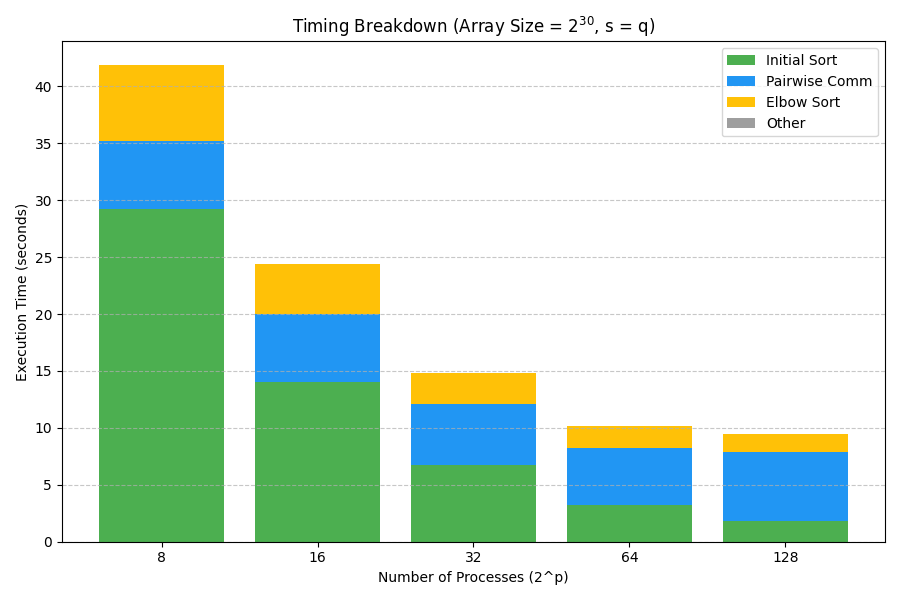
\includegraphics[width=1\linewidth]{figures/stacked_timing.png}
    \caption{Execution time breakdown per stage for total size $2^{27}$ with no buffer splitting ($s = q$).}
    \label{fig:stacked_timing}
\end{figure}

\begin{table}[h]
\centering
\caption{Execution Time Breakdown by Stage (total size: $2^{p+q} = 2^{27},\, s = q$)}
\label{tab:time_breakdown}
\begin{tabular}{|c|c|c|c|c|c|}
\hline
\textbf{p} & \textbf{q} & \textbf{Initial Sort (\%)} & \textbf{Pairwise Sort (\%)} & 
\textbf{Elbow Sort (\%)} & \textbf{Other (\%)} \\
\hline
0 & 27 & \textbf{100.00} & 0.00 & 0.00 & 0.00 \\
1 & 26 & \textbf{92.79} & 2.54 & 4.66 & 0.01 \\
2 & 25 & \textbf{81.27} & 6.79 & 11.93 & 0.01 \\
3 & 24 & \textbf{69.53} & 12.42 & 18.04 & 0.01 \\
4 & 23 & \textbf{58.09} & 21.84 & 20.06 & 0.02 \\
5 & 22 & \textbf{43.02} & 35.50 & 21.45 & 0.03 \\
6 & 21 & 29.92 & \textbf{50.97} & 19.08 & 0.03 \\
7 & 20 & 17.07 & \textbf{66.08} & 16.81 & 0.05 \\
\hline
\end{tabular}
\end{table}

\subsection{Optimizing Pairwise Communication}

As shown in the previous subsection, \textit{pairwise communication} becomes the dominant performance bottleneck 
for large process counts. To mitigate this overhead, we experimented with splitting the communication buffer into
smaller batches. This technique aims to overlap communication with computation and improve scalability.

Figure~\ref{fig:pairwise_comm_vs_procs_splits_sum} shows the impact of different buffer split configurations, 
defined by $B = 2^{q-s}$, on the pairwise communication time. We observe that buffer splitting reduces 
communication time slightly for moderate process counts. However, when the number of processes becomes too large,
splitting becomes counterproductive -- particularly when $p$ is large and $q$ is small, resulting in limited data 
per process. In such cases, the overhead of managing multiple small transfers outweighs any benefits from overlap.

Therefore, while buffer splitting can be marginally beneficial in some configurations, it is not sufficient to 
scale communication performance at large process counts. This observation motivates further work toward optimizing
\textit{local sorting}, which increasingly dominates as communication optimizations saturate.

\begin{figure}
    \centering
    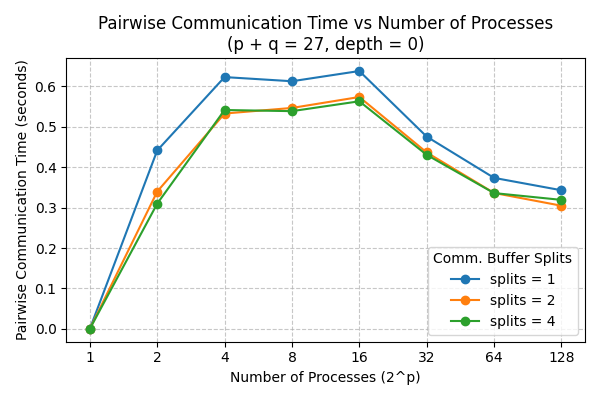
\includegraphics[width=1\linewidth]{figures/pairwise_comm_vs_procs_splits_sum.png}
    \caption{Pairwise communication time vs number of processes for varying communication buffer splits 
    ($B = 2^{q-s}$).}
    \label{fig:pairwise_comm_vs_procs_splits_sum}
\end{figure}

\subsection{Scalability with Respect to Total Data Size}

Finally, Fig.~\ref{fig:total_time_vs_elements} presents the total execution time as a function of the 
total array size for all tested configurations of $p$ and $q$. For each array size $2^{p+q}$, we observe
that increasing the number of processes leads to a consistent reduction in execution time. This clearly 
demonstrates the effectiveness of the parallelization strategy in improving performance as the problem 
size scales.

\begin{figure}[h]
    \centering
    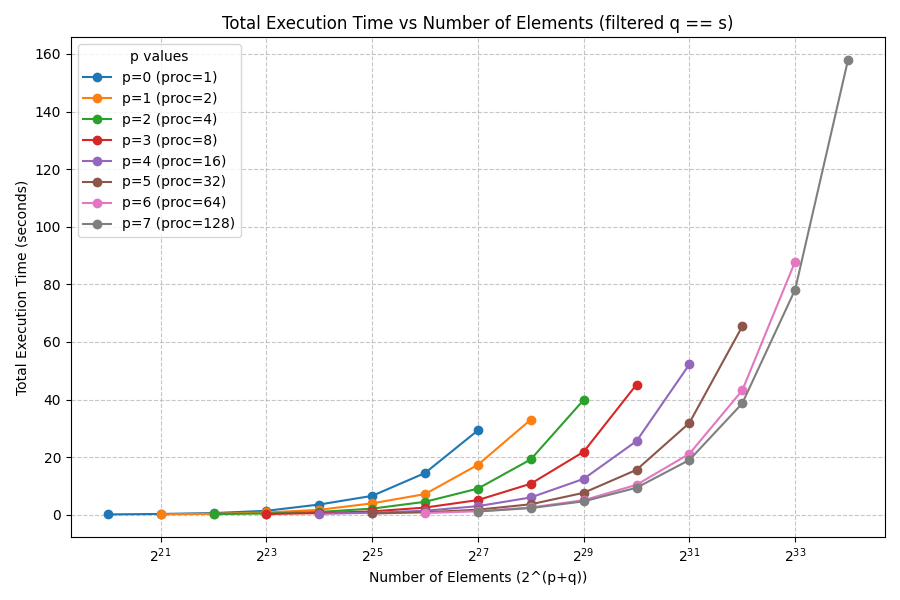
\includegraphics[width=1\linewidth]{figures/total_time_vs_elements.png}
    \caption{Total execution time vs total array size for all $(p, q)$ combinations.}
    \label{fig:total_time_vs_elements}
\end{figure}

\section{Conclusions and Future Work}

In this work, we developed and evaluated a hybrid distributed sorting algorithm that combines local sorting 
with inter-process Bitonic merging. The design leverages the structured nature of Bitonic Sort and the 
communication regularity provided by the hypercube topology formed through bitwise XOR partner selection.

Our benchmarks show that the algorithm scales well with increasing problem size and number of processes. 
When the number of processes is relatively small, performance is limited by the cost of local sorting. 
However, as the number of processes increases, pairwise communication emerges as the dominant bottleneck. 
We explored the effect of buffer splitting as a strategy to mitigate this cost, finding that it provides 
marginal benefits only in specific configurations, and may become counterproductive in high-parallelism 
regimes due to increased message overhead.

Future work will focus on optimizing the local sorting phase by implementing Bitonic Sort on GPUs 
using CUDA. Since Bitonic Sort is inherently parallel and well-suited for GPU architectures, this approach 
can significantly accelerate local sorting, reduce the overall execution time, and better balance the 
computation-communication ratio in the distributed algorithm.

Overall, the results validate that distributed Bitonic Sort can serve as a scalable backbone for parallel 
sorting tasks, provided that communication and local computation are carefully balanced.

\section*{Acknowledgments}

The experiments presented in this work were conducted using the Aristotelis HPC cluster at Aristotle 
University of Thessaloniki (AUTH). We gratefully acknowledge the computational resources and support 
provided by AUTH.


\end{document}
